\subsection{Interpolation by Spline Functions(样条插值)}



\frame{
\frametitle{Interpolation by Spline Functions}
\framesubtitle{样条插值}
\begin{itemize}
\item Polynomial interpolation for a set of $N + 1$ points $\{ (x_k, y_k)\}^N_{k=0}$ is frequently unsatisfactory. 
\vspace{0.3cm}
\item A polynomial of degree $N$ can have $N -1$ relative maxima and minima, and the graph can wiggle in order to pass through the points. 
\vspace{0.3cm}
\item Another method is to piece together the graphs of lower-degree polynomials $S_k(x)$ and interpolate between the successive nodes $(x_k, y_k)$ and $(x_{k+1}, y_{k+1})$ . 
\end{itemize}
}

\frame{
\begin{figure}
\begin{center}
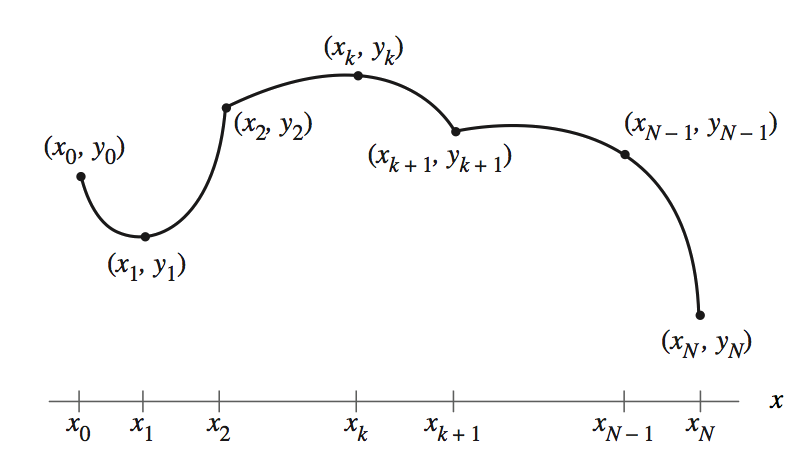
\includegraphics[width=70mm]{chap-4/fig_5-10.png}
\end{center}
\end{figure}
\begin{itemize}
\item The two adjacent portions of the curve $y = S_k(x)$ and $Y = S_{k+1}(x)$, which lie above $[x_k, x_{k+1}]$ and $[x_{k+1}, x_{k+2}]$, respectively, pass through the common {\Large knot} $(x_{k+1}, y_{k+1})$. 
\item The two portions of the graph are tied together at the knot $(x_{k+1}, y_{k+1})$, and the set of functions $\{ S_k(x) \}$ forms a piecewise polynomial curve, which is denoted by $S(x)$. 
\end{itemize}
}



\frame{
\frametitle{Piecewise Linear Interpolation}
\framesubtitle{分段线性插值}
The simplest polynomial to use, a polynomial of degree 1, produces a polygonal path that consists of line segments that pass through the points.  
The Lagrange polynomial  is used to represent this piecewise linear curve:
\begin{equation*}
S_k(x) = y_k \frac{x-x_{k+1}}{x_k-x_{k+1}} + y_{k+1} \frac{x-x_k}{x_{k+1}-x_k}
\end{equation*}
The resulting curve looks like a broken line (see Figure 4.11). 
\begin{figure}
\begin{center}
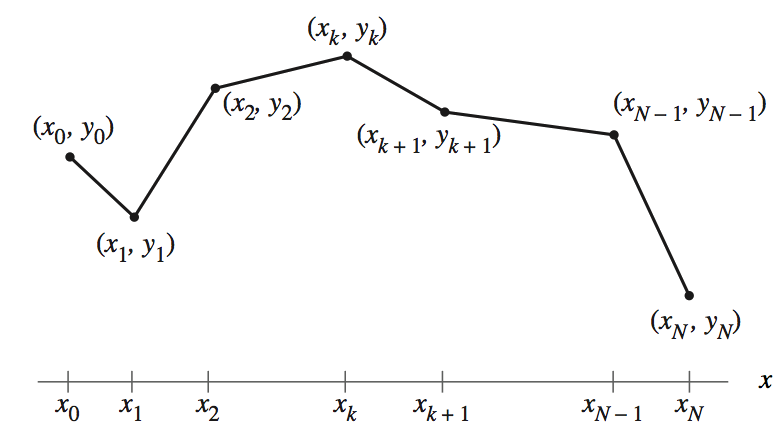
\includegraphics[width=60mm]{chap-4/fig_5-11.png}
\end{center}
\end{figure}
}


\frame{
An equivalent expression can be obtained if we use the point-slope formula for a line segment: 
\begin{equation*}
S_k(x) = y_k + d_k (x - x_k)
\end{equation*}
where $d_k = (y_{k+1} - y_k) / (x_{k+1} - x_k)$. 
The resulting {\Large linear spline} function can be written in the form 
\begin{equation*}
S(x) = \left\{
\begin{array}{l l}
y_0 + d_0(x-x_0) & for \ x \ in \ [x_0, x_1] \\
y_1 + d_1(x-x_1) & for \ x \ in \ [x_1, x_2] \\
\vdots & \vdots \\
y_k + d_k(x-x_k) & for \ x \ in \ [x_k, x_{k+1}] \\
\vdots & \vdots \\
y_{N-1} + d_{N-1}(x-x_{N-1}) & for \ x \ in \ [x_{N-1}, x_N] 
\end{array}
\right.
\end{equation*}
}

\frame{
\begin{itemize}
\item It is assumed that the abscissas are ordered $x_0 < x_1 < \ldots < x_{N-1} < x_N$. 
\vspace{0.3cm}
\item For a fixed value of $x$, the interval $[x_k, x_{k+1}]$ containing {x} can be found by successively computing the differences $x - x_1, \ldots , x - x_k, x - x_{k+1}$ until $k + 1$ is the smallest integer such that $x - x_{k+1} < 0$. 
\vspace{0.3cm}
\item Hence we have found $k$ so that $x_k \le x \le  x_{k+1}$, and the value of the spline function $S(x)$ is 
\begin{equation*}
S(x) = S_k(x) = y_k + d_k(x-x_k)  \ \ \ \ for \ x_k \le x \le  x_{k+1}
\end{equation*}
\end{itemize}
}

\frame{
These techniques can be extended to higher-order polynomials.  \\
\vspace{0.3cm}
For example, if an odd number of nodes $x_0, x_1, \ldots , x_{2M}$ is given, then a piecewise quadratic polynomial can be constructed on each subinterval $[x_{2k}, x_{2k+2}]$, for $k = 0,1, \ldots ,M - 1$. 
\begin{itemize}
\item A shortcoming of the resulting quadratic spline\footnote{二次样条} is that the curvature at the even nodes $x_{2k}$ changes abruptly, and this can cause an undesired bend or distortion in the graph. 
\item The second derivative of a quadratic spline is discontinuous at the even nodes. 
\end{itemize}
\begin{block}{}
If we use piecewise cubic polynomials, then both the first and second derivatives can be made continuous. 
\end{block}
}

\frame{
\frametitle{Piecewise Cubic Splines}
\framesubtitle{分段三次样条}
\begin{itemize}
\item The fitting of a polynomial curve to a set of data points has applications in CAD (computer-assisted design), CAM (computer-assisted manufacturing), and computer graphics systems. 
\vspace{0.3cm}
\item An operator wants to draw a smooth curve through data points that are not subject to error. 
\vspace{0.3cm}
\item Traditionally, it was common to use a french curve\footnote{曲线板,云尺} or an architect's spline and subjectively draw a curve that looks smooth when viewed by the eye. 
\end{itemize}
}

\frame{
Mathematically, it is possible to construct cubic functions $S_k(x)$ on each interval $[x_k, x_{k+1}]$ so that the resulting piecewise curve $y = S(x)$ and its first and second derivatives are all continuous on the larger interval $[x_0,x_N]$. 
\begin{itemize}
\vspace{0.5cm}
\item The continuity of $S'(x)$ means that the graph $y = S(x)$ will not have sharp corners. 
\vspace{0.3cm}
\item The continuity of $S"(x)$ means that the {\Large radius of curvature} is defined at each point. 
\end{itemize}
}

\frame{
\begin{block}{Definition}
Suppose that $\{ (x_k, y_k)\}_{ k=0}^N$ are $N + 1$ points, where $a = x_0 < x_1 < \cdots < x_N = b$. 
The function $S(x)$ is called a {\Large cubic spline} if there exist $N$ cubic polynomials $S_k(x)$ with coefficients $s_{k,0}$, $s_{k,1}$, $s_{k,2}$, and $s_{k,3}$ that satisfy the following properties:
\begin{equation*}
\begin{array}{l}
I.  S(x) = S_k(x) = s_{k,0} + s_{k,1}(x - x_k) + s_{k,2}(x - x_k)^2 + s_{k,3}(x - x_k)^3 \\
  for \  x \in [x_k , x_{k+1}] \  and \ k = 0, 1, \ldots , N - 1. \\ \\
\begin{array}{l l l}
II.  & S(x_k)= y_k & for \ k = 0,1,\ldots, N \\
& & \\
III. & S_k(x_{k+1})=S_{k+1}(x_{k+1}) & for \ k=0,1,\ldots,N-2. \\
& & \\
IV. & S_k′(x_{k+1})=S′_{k+1}(x_{k+1}) &  for \ k=0,1,\ldots,N-2. \\
& & \\
V.  & S_k′′(x_{k+1})=S′′_{k+1} (x_{k+1}) &  for \ k=0,1,\ldots,N-2. \\
\end{array}
\end{array}
\end{equation*}
\end{block}
}

\frame{
\frametitle{Property of Cubic Spline}
\begin{itemize}
\item Property I states that $S(x)$ consists of piecewise cubics. 
\vspace{0.3cm}
\item Property II states that the piecewise cubics interpolate the given set of data points. 
\vspace{0.3cm}
\item Properties III and IV require that the piecewise cubics represent ,a smooth continuous function. 
\vspace{0.3cm}
\item Property V states that the second derivative of the resulting function is also continuous. 
\end{itemize}
}

\frame{
\frametitle{Existence of Cubic Splines}
Let us try to determine if it is possible to construct a cubic spline that satisfies properties I through V. 
\begin{itemize}
\item Each cubic polynomial $S_k(X)$ has four unknown constants ($s_{k,0}$, $s_{k,1}$, $s_{k,2}$, and $s_{k,3}$); hence there are $4N$ coefficients to be determined. 
\item Loosely speaking, we have $4N$ degrees of freedom or conditions that must be specified. 
\item The data points supply $N + 1$ conditions, and properties III, IV, and each supply $N - 1$ conditions.  Hence, $N + 1 + 3(N - 1) = 4N - 2$ conditions are specified. 
\item This leaves us two additional degrees of freedom. 
\end{itemize}
\begin{block}{}
We will call them {\Large endpoint constraints}: they will involve either $S'(x)$ or $S"(x)$ at $x_0$ and $x_N$ and will be discussed later. 
\end{block}
}

\frame{
Since $S(x)$ is piecewise cubic, its second derivative $S"(x)$ is piecewise linear on $[x_0, x_N]$. 
The linear Lagrange interpolation formula gives the following representation for $S"(x) = S"_k(x)$: 
\begin{equation*}
S"(x) = S"(x_k) \frac{x - x_{k+1}}{x_k-x_{k+1}} + S"(x_{k+1}) \frac{x-x_k}{x_{k+1}-x_k}
\end{equation*}
Use $m_k = S"(x_k)$, $m_{k+1} = S"(x_{k+1})$, and $h_k = x_{k+1} - x_k$ in (4.53) to get
\begin{equation*}
S"(x) = \frac{m_k}{h_k}(x_{k+1}-x) + \frac{m_{k+1}}{h_k}(x-x_k)
\end{equation*}
for $x_k \le x \le x_{k+1}$ and $k = 0,1, ... , N -1$. 
}

\frame{
Integrating  twice will introduce two constants of integration, and the result can be manipulated so that it has the form
\begin{equation*}
S_k(x) = \frac{m_k}{6h_k}  (x_{k+1} - x)^3 + \frac{m_{k+1}}{6h_k} (x - x_k)^3	+p_k (x_{k+1} - x) + q_k(x - x_k).
\end{equation*}
Substituting $x_k$ and $x_{k+1}$ into the above equation  and using the values $y_k = S_k(x_k)$ and $y_{k+1} = S_k(x_{k+1})$ yields the following equations that involve $p_k$ and $q_k$, respectively: 
\begin{equation*}
y_k = \frac{m_k}{6} h_k^2 + p_k h_k
\end{equation*}
and 
\begin{equation*}
y_{k+1} = \frac{m_{k+1}}{6} h_k^2 + q_k h_k
\end{equation*}
}


\frame{
These two equations are easily solved for $p_k$ and $q_k$, and when these values are substituted into the above equations, the result is the following expression for the cubic function $S_k(x)$:
\begin{equation*}
\begin{array}{l l}
s_k(x) = &  - \frac{m_k}{6h_k} (x_{k+1}-x)^3 + \frac{m_{k+1}}{6h_k}(x-x_k)^3 \\
& \\
& \left( \frac{y_k}{h_k} - \frac{m_k h_k}{6} \right) (x_{k+1} -x) + \left(  \frac{y_{k+1}}{h_k} - \frac{m_{k+1} h_k}{6} \right) (x - x_k) 
\end{array}
\end{equation*}
Notice that the representation has been reduced to a form that involves only the unknown coefficients $\{ m_k \}$. 
To find these values, we must use the derivative, which is 
\begin{equation*}
\begin{array}{l l}
s'_k(x) = &  - \frac{m_k}{2h_k} (x_{k+1}-x)^2 + \frac{m_{k+1}}{2h_k}(x-x_k)^2 \\
& \\
& + \left( \frac{y_k}{h_k} - \frac{m_k h_k}{6} \right) + \left( \frac{y_{k+1}}{h_k} - \frac{m_{k+1} h_k}{h_k} \right)
\end{array}
\end{equation*}
}

\frame{
Evaluating  at $x_k$ and simplifying the result yield
\begin{equation*}
S'_k (x_k) = - \frac{m_k}{3} h_k - \frac{m_{k+1}}{6}h_k + d_k
\end{equation*}
where
\begin{equation*}
d_k = \frac{y_{k+1} - y_k}{h_k}
\end{equation*}
Similarly, we can replace $k$ by $k -1$ in above equation to get the expression for $S'_{k-1}(x)$ and evaluate it at $x_k$ to obtain 
\begin{equation*}
S'_{k-1} (x_k) = \frac{m_k}{3} h_{k-1} + \frac{m_{k-1}}{6} + d_{k-1}
\end{equation*}
}

\frame{
Now use property IV  to obtain an important relation involving $m_{k-1}$, $m_k$, and $m_{k+1}$: 
\begin{equation*}
h_{k-1} m_{k-1} + 2 (h_{k-1} + h_k) m_k + h_k m_{k+1} = u_k
\end{equation*}
where 
\begin{equation*}
u_k = 6 ( d_k - d_{k-1} )
\end{equation*}
for $k = 0,1, \ldots , N - 1$
}




\frame{
\frametitle{Construction of Cubic Splines}
\begin{itemize}
\item Observe that the unknowns in above equation are the desired values $\{ m_k\}$, and the other terms are constants obtained by performing simple arithmetic with the data points $\{ (x_k, y_k)\}$. 
\item Therefore, in reality, system  is an under determined system of $N - 1$ linear equations involving $N + 1$ unknowns. 
\item Hence two additional equations must be supplied. 
\item They are used to eliminate $m_0$ from the first equation and $m_N$ from the $(N - l)$-st equation in system . 
\end{itemize}
}

\frame{
The standard strategies for the endpoint constraints are summarized in the following table.
\begin{figure}
\begin{center}
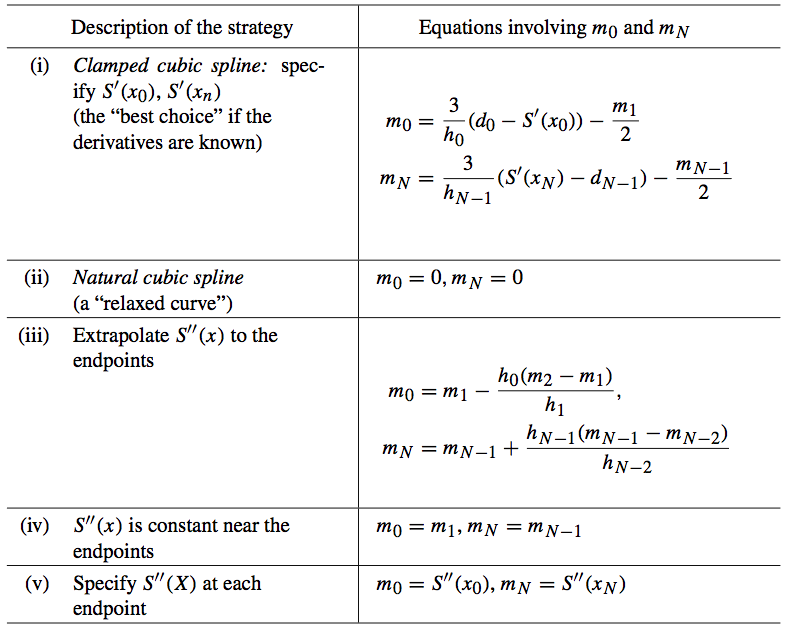
\includegraphics[width=90mm]{chap-4/tab_5-8.png}
\end{center}
\end{figure}
}

\frame{
Consider strategy (v) in Table. 
If $m_0$ is given, then $h_0m_0$ can be computed, and the first equation (when $k = 1$)  is 
\begin{equation*}
2 \left( h_0 + h_1 \right) m_1 + h_1 m_2 = u_1 - h_0 m_0
\end{equation*}
Similarly, if $m_N$ is given, then $h_{N-1}m_N$ can be computed, and the last equation (when $k = N - 1$) of (4.61) is 
\begin{equation*}
h_{N-2} m _{N-2} + 2 \left( h_{N-2} + h_{N-1} \right) m_{N-1} = u_{N-1} - h_{N-1}m_N
\end{equation*}
Equations  used for $k = 2,3, ... ,N - 2$ form $N - 1$ linear equations involving the coefficients $m_1, m_2, \ldots , m_{N-l}$ 
}

\frame{
Regardless of the particular strategy chosen in the table, we can rewrite equations $1$ and $N - 1$  and obtain a tridiagonal linear system of the form $HM = V$, which involves $m_1, m_2, \ldots, m_{N-1}$: 
\begin{equation*}
\left[ 
\begin{array}{c c c c c c}
b_1 & c_1 & & & & \\
a_1 & b_2 & c_2 & & & \\
& & \ddots & & & \\
& & & a_{N-3} & b_{N-2} & c_{N-2} \\
& & & & a_{N-2} & b_{N-1}
\end{array}
\right] 
\left[ 
\begin{array}{c}
m_1 \\
m_2 \\
\cdots \\
m_{N-2} \\
m_{N-1}
\end{array}
\right] 
= 
\left[ 
\begin{array}{c}
v_1 \\
v_2 \\
\cdots \\
v_{N-2} \\
v_{N-1}
\end{array}
\right]
\end{equation*}
}

\frame{
The linear system  is strictly diagonally dominant and has a unique solution . 
After the coefficients $\{ m_k \}$ are determined, the spline coefficients $\{s_{k,j}\}$ for $S_k(x)$ are computed using the formulas 
\begin{equation*}
\begin{array}{l l}
s_{k,0} = y_k & s_{k,1} = d_k - \%frac{h_k(2m_k+m_{k+1})}{6} \\
& \\
s_{k,2} = \frac{m_k}{2} & s_{k,3} = \frac{m_{k+1}-m_k}{6h_k}
\end{array}
\end{equation*}
Each cubic polynomial $S_k(x)$ can be written in nested multiplication form for efficient computation: 
\begin{equation*}
S_k(x) = \left( \left( s_{k,3}w + s_{k,2} \right) w + s_{k,1} \right) w + y_k, \ \ \ where \ w =x - x_k
\end{equation*}
and $S_k(x)$ is used on the interval $x_k \le x \le x_{k+1}$. 
}

%\frame{
%\begin{itemize}
%\item Equations (4.61) together with a strategy from Table 4.8 can be used to construct a cubic spline with distinctive properties at the endpoints.
%\item Specifically, the values for $m_0$ and $m_N$ in Table 4.8 are used to customize the first and last equations in (4.61) and form the system of $N - 1$ equations given in (4.64). 
%\item Then the tridiagonal system is solved for the remaining coefficients $m_1$, $m_2$, $\ldots$ , $m_{N-1}$. 
%\item Finally, the formulas in (4.65) are used to determine the spline coefficients. 
%\end{itemize}
%}

\frame{
\frametitle{Endpoint Constraints}
The following five lemmas show the form of the tridiagonal linear system that must be solved for each of the different endpoint constraints in the above table. 
}

\frame{
\begin{block}{Lemma 1 (Clamped Spline 固定样条)}
There exists a unique cubic spline with the first derivative boundary conditions $S′(a) = d_0$ and $S′(b) = d_N$ .
\end{block}
\vspace{0.3cm}
Proof. \\
Solve the linear system
\begin{equation*}
\begin{array}{r l}
\left( \frac{3}{2} h_0 + 2 h_1\right) m_1 + h_1 m_2 & = u_1 - 3 (d_0 - S'(x_0)) \\
& \\
h_{k-1}m_{k-1}+2(h_k-1+h_k)m_k+h_km_{k+1} & = u_k \ \ \ for \  k=2, 3, \ldots, N-2 \\
& \\
h_{N-2}m_{N-2} + \left( 2h_{N-2}+\frac{3}{2}h_{N-1} \right) m_{N-1} & = u_{N-1} - 3(S′(x_N)-d_{N-1}).
\end{array}
\end{equation*}
}


\frame{
\begin{block}{Remark of Lemma 1.}
\begin{itemize}
\item The clamped spline involves slope at the ends. 
\vspace{0.3cm}
\item This spline can be visualized  as the curve obtained when a flexible elastic rod is forced to pass through the data points, and the rod is clamped at each end with a fixed slope. 
\vspace{0.3cm}
\item This spline would be useful to a draftsman for drawing a smooth curve through several points. 
\end{itemize}
\end{block}
}

\frame{
\begin{block}{Lemma 2 (Natural Spline自然样条)}
There exists a unique cubic spline with the free boundary conditions $S′′(a) = 0$ and $S′′(b) = 0$.
\end{block}
\vspace{0.3cm}
Proof. \\
Solve the linear system
\begin{equation*}
\begin{array}{r l}
2(h_0 + h_1) m+1 + h_1m_2 & = u_1 \\
& \\
h_{k-1}m_{k-1} + 2 (h_{k-1}+h_k)m_k + h_km_{k+1} & = u_k \ \ \ for \ k=2, 3, \ldots, N-2. \\
& \\
h_{N-2}m_{N-2} + 2(h_{N-2} + h_{N-1})m_{N-1} & = u_{N-1}.
\end{array}
\end{equation*}
}

\frame{
\begin{block}{Remark of Lemma 2.}
\begin{itemize}
\item The natural spline is the curve obtained by forcing a flexible elastic rod  through the data points but letting the slope at the ends be free to equilibrate to the position that minimizes the oscillatory behavior of the curve. 
\vspace{0.3cm}
\item It is useful for fitting a curve to experimental data that are significant to several significant digits. 
\end{itemize}
\end{block}
}

\frame{
\begin{block}{Lemma 3 (Extrapolated Spline 外延样条).}
There exists a unique cubic spline that uses extrapolation from the interior nodes at $x_1$ and $x_2$ to determine $S''(a)$ and extrapolation from the nodes at $x_{N-1}$ and $x_{N-2}$ to determine $S''(b)$.
\end{block}
Proof. \\
Solve the linear system
\begin{equation*}
\begin{array}{r l}
\left( 3 h_0 + 2 h_1+\frac{h_0^2}{h_1} \right) m_1+ \left( h_1− \frac{h^2_0}{h_1} \right) m_2 & = u_1 \\
& \\
h_{k-1} m_{k-1} + 2 (h_{k-1} + h_k) m_k + h_km_{k+1} & = u_k \\
&  for \ k = 2,3,\ldots N-2\\
& \\
\left( h_{N-2} -	\frac{h_{N-1}^2}{h_{N-2}} \right) m_{N-2} +	\left( 2h_{N-2} + 3h_{N-1} + \frac{h_{N-1}^2}{h_{N-2}} \right) m_{N-1} & = u_{N-1} 
\end{array}
\end{equation*}
}

\frame{
\begin{block}{Remark of Lemma 3}
The extrapolated spline is equivalent to assuming that the end cubic is an extension of the adjacent cubic;  \\
\vspace{0.3cm}
that is, the spline forms a single cubic curve over the interval $[x_0, x_2]$ and another single cubic over the interval $[x_{N-2}, x_N]$. 
\end{block}
}

\frame{
\begin{block}{Lemma 4 (Parabolically Terminated Spline).}
There exists a unique cubic spline that uses $S'''(x) \equiv 0$ on the interval $[x_0, x_1]$ and $S'''(x) ≡ 0$ on $[x_{N-1}, x_N ]$.
\end{block}
Proof. \\
Solve the linear system
\begin{equation*}
\begin{array}{r l}
(3h_0 + 2h_1) m_1 + h_1m_2 & = u_1 \\ 
h_{k-1}m_{k-1} + 2(h_{k-1} + h_k)m_k + h_k m_k+1 & =u_k \ \ \	for \ k=2, 3, \ldots, N-2 \\
h_{N-2}m_{N-2} + (2h_{N-2} + 3h_{N-1})m_{N-1} = u_{N-1}.	
\end{array}
\end{equation*}
\begin{block}{Remark.}
The assumption that $S"(x) \equiv 0$ on the interval $[x_0, x_1]$ forces the cubic to degenerate to a quadratic over $[x_0, x_1]$, and a similar situation occurs over $[x_{N-1}, x_N]$. 
\end{block}
}

\frame{
\begin{block}{Lemma 5 (Endpoint Curvature-Adjusted Spline).}
There exists a unique cubic spline with the second derivative boundary conditions $S′′(a)$ and $S′′(b)$ specified.
\end{block}
Proof. \\
Solve the linear system
\begin{equation*}
\begin{array}{r l}
2(h_0 + h_1) m_1 + h_1 m_2 & = u_1 - h_0 S′′(x_0) \\ 
h_{k-1}m_{k-1}+2(h_{k-1}+h_k)m_k + h_km_{k+1} & = u_k \ \ \ for \  k = 2, 3, \ldots, N-2 \\
h_{N-2}m_{N-2} +2(h_{N-2} +h_{N-1})m_{N-1} & = u_{N-1} −h_{N-1} S′′(x_N).
\end{array}
\end{equation*}
\begin{block}{Remark.}
Imposing values for $S"(a)$  and $S"(b)$ permits the practitioner to adjust the curvature at each endpoint. 
\end{block}
}


\frame{
\frametitle{Example} 
Find the clamped cubic spline that passes through $(0, 0)$, $(1, 0.5)$, $(2, 2.0)$, and $(3, 1.5)$ with the first derivative boundary conditions $S'(0) = 0.2$ and $S'(3) = -1$.

First, compute the quantities
\begin{equation*}
\begin{array}{l c l}
h_0 & = & h_1 = h_2 = 1 \\
d_0 & = & (y_1 - y_0) \slash h_0 = (0.5 - 0.0) \slash 1 = 0.5 \\
d_1 & = & (y_2 - y_1) \slash h_1 = (2.0 - 0.5) \slash 1 = 1.5 \\
d_2 & = & (y_3 - y_2) \slash h_2 = (1.5 - 2.0) \slash 1 = -0.5 \\
u_1 & = & 6(d_1 - d_0) = 6(1.5 - 0.5) = 6.0 \\
u_2 & = & 6(d_2 - d_1) = 6(-0.5 - 1.5) = -12.0.
\end{array}
\end{equation*}
Then use Lemma 4.1 and obtain the equations
\begin{equation*}
\left( \frac{3}{2} + 2 \right) m_1 + m_2 = 6.0 - 3(0.5 - 0.2) = 5.1,
\end{equation*}
\begin{equation*}
m_1 +  \left( 2 + \frac{3}{2} \right) m_2 = -12.0 - 3(-1.0 - (-0.5)) = -10.5.
\end{equation*}
}

\frame{
When these equations are simplified and put in matrix notation, we have
\begin{equation*}
\left[ 
\begin{array}{c c}
3.5 & 1.0 \\
1.0 & 3.5
\end{array}
\right]
\left[ 
\begin{array}{c}
m_1 \\
m_2
\end{array}
\right]
=
\left[ 
\begin{array}{c}
5.1 \\
-10.5
\end{array}
\right]
\end{equation*}
It is a straightforward task to compute the solution $m_1 = 2.25$ and $m_2 = -3.72$. 
Now apply the equations in (i) of Table 4.8 to determine the coefficients $m_0$ and $m_3$:
\begin{equation*}
m_0 = 3(0.5 - 0.2) - \frac{2.52}{2} = - 0.36
\end{equation*}
\begin{equation*}
m_3 = 3(-1.0 + 0.5) - \frac{-3.72}{2} = 0.36
\end{equation*}
}

\frame{
Next, the values $m_0 = -0.36$, $m_1 = 2.25$, $m_2 = -3.72$, and $m_3 = 0.36$ are substituted into equations (4.65) to find the spline coefficients. 

The solution is
\begin{equation*}
\begin{array}{l c l l}
S_0(x) & = & 0.48x^3 - 0.18x^2 + 0.2x & for \ \ \ 0 \le x \le 1, \\
S_1(x) & = & -1.04(x - 1)^3 + 1.26(x - 1)^2 & \\
& & + 1.28(x - 1) + 0.5 & for \ \ \ 1 \le x \le 2, \\
S_2(x) & = & 0.68(x - 2)^3 - 1.86(x - 2)^2 & \\
& & + 0.68(x - 2) + 2.0 & for \ \ \ 2 \le x \le 3.
\end{array}
\end{equation*}
\begin{figure}
\begin{center}
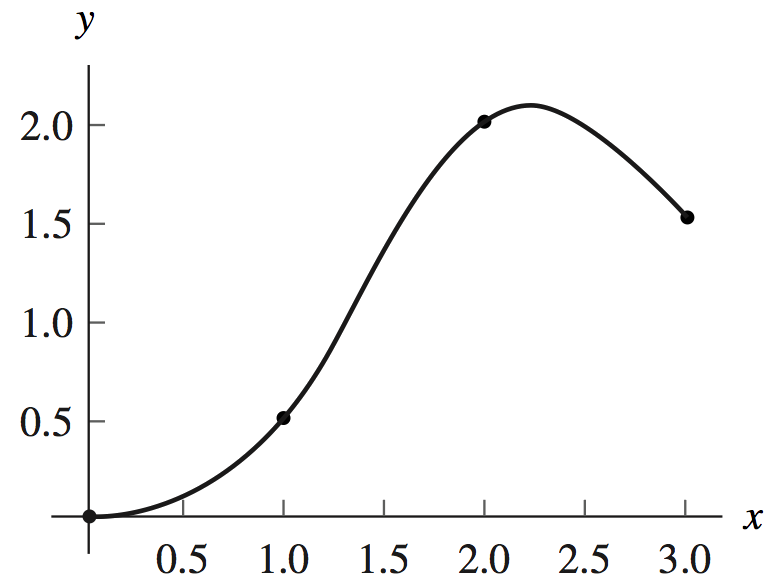
\includegraphics[width=40mm]{chap-4/fig_5-12.png}
\end{center}
\end{figure}
}

\frame{
\frametitle{Example }
Find the natural cubic spline that passes through $(0, 0.0)$, $(1, 0.5)$, $(2, 2.0)$, and $(3, 1.5)$ with the free boundary conditions $S''(x) = 0$ and $S''(3) = 0$.

Use the same values $\{ h_k \}$, $\{ d_k \}$, and $\{ u_k \}$ that were computed in Example 4.7. 
Then use Lemma 4.2 and obtain the equations
\begin{equation*}
2(1 + 1)m_1 + m_2 = 6.0,
\end{equation*}
\begin{equation*}
m_1 + 2(1 + 1)m_2 = -12.0.
\end{equation*}
The matrix form of this linear system is
\begin{equation*}
\left[ 
\begin{array}{c c}
4.0 & 1.0 \\
1.0 & 4.0
\end{array}
\right]
\left[ 
\begin{array}{c}
m_1 \\
m_2
\end{array}
\right]
=
\left[ 
\begin{array}{c}
6.0 \\
-12.0
\end{array}
\right]
\end{equation*}
It is easy to find the solution $m_1 = 2.4$ and $m_2 = -3.6$. 
}

\frame{
Since $m_0= S''(0) = 0$ and $m_3 = S''(3) = 0$, 
when equations  are used to find the spline coefficients, the result is
\begin{equation*}
\begin{array}{l c l l}
S_0(x) & = & 0.4 x^3 + 0.1x^2  & for \ \ \ 0 \le x \le 1, \\
S_1(x) & = & -(x - 1)^3 + 1.2(x - 1)^2 & \\
& & + 1.3(x - 1) + 0.5 & for \ \ \ 1 \le x \le 2, \\
S_2(x) & = & 0.6(x - 2)^3 - 1.8(x - 2)^2 & \\
& & + 0.7(x - 2) + 2.0 & for \ \ \ 2 \le x \le 3.
\end{array}
\end{equation*}
\begin{figure}
\begin{center}
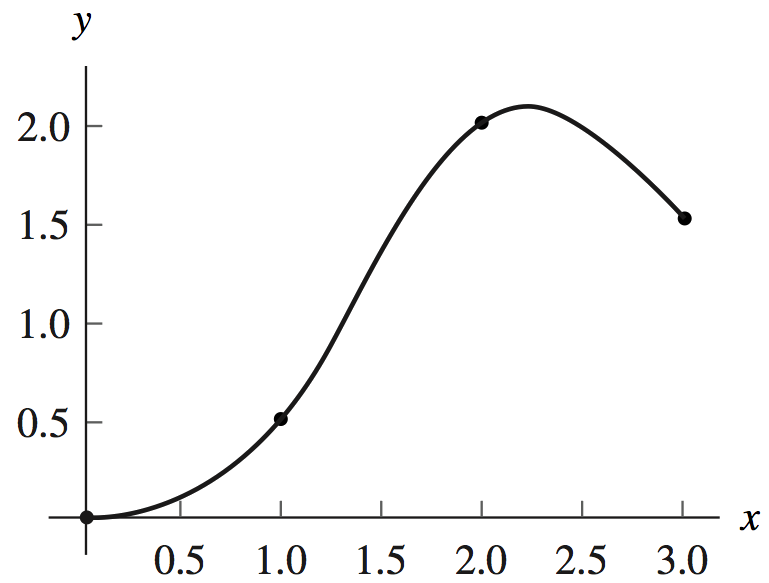
\includegraphics[width=40mm]{chap-4/fig_5-13.png}
\end{center}
\end{figure}
}



\frame{
\frametitle{Example.} 
Find the extrapolated cubic spline through $(0, 0.0)$, $(1, 0.5)$, $(2, 2.0)$, and $(3, 1.5)$.

Use the values $\{h_k\}$, $\{d_k\}$, and $\{u_k\}$ from Example 4.7 with Lemma 3 and obtain the linear system
\begin{equation*}
(3 + 2 + 1) m_1 + (1 - 1) m_2 = 6.0,
\end{equation*}
\begin{equation*}
(1 - 1) m_1 + (2 + 3 + 1) m_2 = -12.0.
\end{equation*}
The matrix form is
\begin{equation*}
\left[ 
\begin{array}{c c}
6.0 & 0.0 \\
0.0 & 6.0
\end{array}
\right]
\left[ 
\begin{array}{c}
m_1 \\
m_2
\end{array}
\right]
=
\left[ 
\begin{array}{c}
6.0 \\
-12.0
\end{array}
\right]
\end{equation*}
and it is trivial to obtain $m_1 = 1.0$ and $m_2 = -2.0$. 
Now apply the equations in (iii) of Table to compute $m_0$ and $m_3$:
\begin{equation*}
m_0 = 1.0 - (-2.0 - 1.0) = 4.0,
\end{equation*}
\begin{equation*}
m_3 = -2.0 + (-2.0 - 1.0) = -5.0
\end{equation*}
}

\frame{
Finally, the values for $\{m_k\}$ are substituted  to find the spline coefficients.
The solution is
\begin{equation*}
\begin{array}{l c l l}
S_0(x) & = & -0.5 x^3 + 2.0x^2 - x & for \ \ \ 0 \le x \le 1, \\
S_1(x) & = & -0.5 (x - 1)^3 + 0.5 (x - 1)^2 & \\
& & + 1.5(x - 1) + 0.5 & for \ \ \ 1 \le x \le 2, \\
S_2(x) & = & -0.5 (x - 2)^3 - (x - 2)^2 & \\
& & + (x - 2) + 2.0 & for \ \ \ 2 \le x \le 3.
\end{array}
\end{equation*}

\begin{figure}
\begin{center}
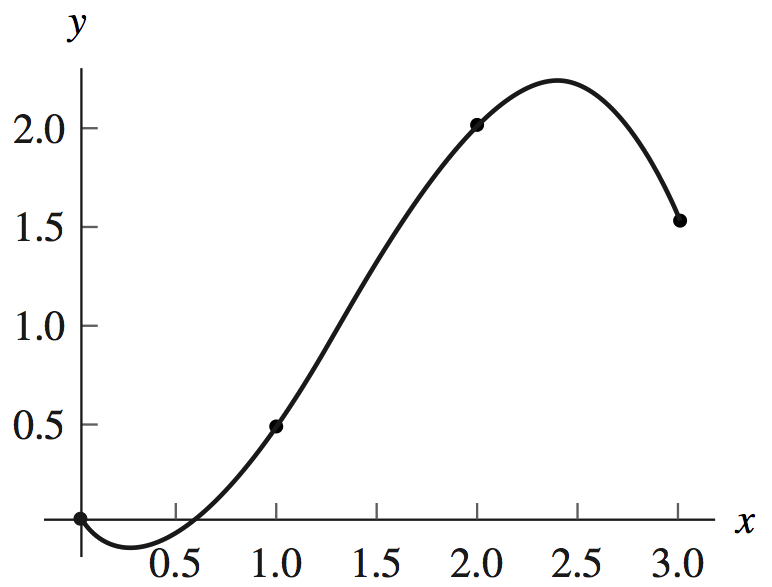
\includegraphics[width=40mm]{chap-4/fig_5-14.png}
\end{center}
\end{figure}
}



\frame{
\frametitle{Example } 
Find the parabolically terminated cubic spline through $(0, 0.0)$, $(1, 0.5)$, $(2, 2.0)$, and $(3, 1.5)$.

Use $\{ h_k \}$, $\{ d_k \}$, and $\{ u_k \}$ from Example  and then apply Lemma 4 to obtain
\begin{equation*}
(3 + 2) m_1 + m_2 = 6.0,
\end{equation*}
\begin{equation*}
m_1 + (2 + 3) m_2 = -12.0.
\end{equation*}
The matrix form is
\begin{equation*}
\left[ 
\begin{array}{c c}
5.0 & 0.0 \\
0.0 & 5.0
\end{array}
\right]
\left[ 
\begin{array}{c}
m_1 \\
m_2
\end{array}
\right]
=
\left[ 
\begin{array}{c}
6.0 \\
-12.0
\end{array}
\right]
\end{equation*}
and the solution is $m_1 = 1.75$ and $m_2 = -2.75$. 
}

\frame{
Since $S''(x) ≡ 0$ on the subinterval at each end, formulas (iv) in Table 4.8 imply that we have $m_0 = m_1 = 1.75$ and $m_3 = m_2 =
-2.75$. 
Then the values for $\{ m_k \}$ are substituted in equations (4.65) to get the solution
\begin{equation*}
\begin{array}{l c l l}
S_0(x) & = & 0.875 x^2 - 0.375 x & for \ \ \ 0 \le x \le 1, \\
S_1(x) & = & -0.75 (x - 1)^3 + 0.875 (x - 1)^2 & \\
& & + 1.375 (x - 1) + 0.5 & for \ \ \ 1 \le x \le 2, \\
S_2(x) & = & -1.375 (x - 2)^2 + 0.875 (x - 2)  + 2.0 & for \ \ \ 2 \le x \le 3.
\end{array}
\end{equation*}

\begin{figure}
\begin{center}
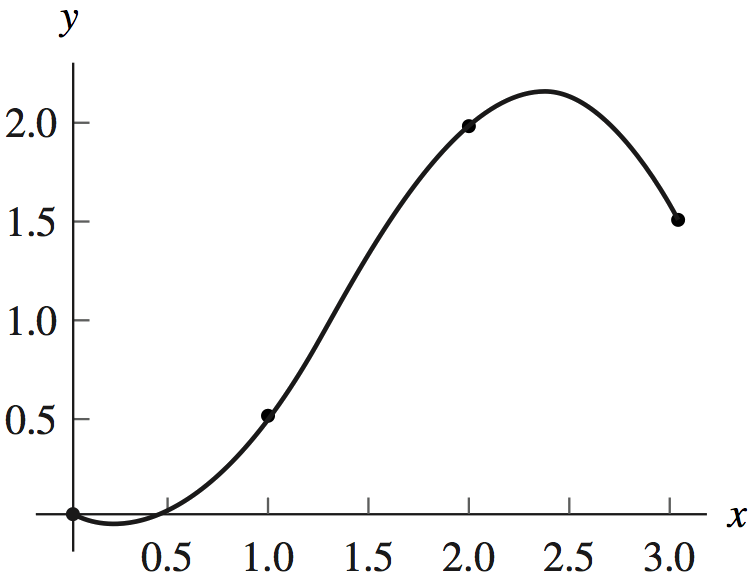
\includegraphics[width=40mm]{chap-4/fig_5-15.png}
\end{center}
\end{figure}
}


\frame{
\frametitle{Example} 
Find the curvature-adjusted cubic spline through $(0, 0.0)$, $(1, 0.5)$, $(2, 2.0)$, and $(3, 1.5)$ with the second derivative boundary conditions  $ S''(0) = -0.3$ and $S''(3) = 3.3$.

Use $\{ h_k \}$, $\{ d_k \}$, and $\{ u_k \}$ from Example 4.7 and then apply Lemma 5 to obtain
\begin{equation*}
2 (1 + 1) m_1 + m_2 = 6.0 - (-0.3) = 6.3,
\end{equation*}
\begin{equation*}
m_1 + 2 (1 + 1) m_2 = -12.0 - (3.3) = -15.3.
\end{equation*}
The matrix form is
\begin{equation*}
\left[ 
\begin{array}{c c}
4.0 & 1.0 \\
1.0 & 4.0
\end{array}
\right]
\left[ 
\begin{array}{c}
m_1 \\
m_2
\end{array}
\right]
=
\left[ 
\begin{array}{c}
6.3 \\
−15.3
\end{array}
\right]
\end{equation*}
and the solution is $m_1 = 2.7$ and $m_2 = -4.5$. 
}

\frame{
The given boundary conditions are used to determine $m_0 = S''(0) = -0.3$ and $m_3 = S''(3) = 3.3$. 

Substitution of $\{ m_k \}$ in equations (4.65) produces the solution


\begin{equation*}
\begin{array}{l c l l}
S_0(x) & = & 0.5 x^3 - 0.15 x^2 + 0.15 x & for \ \ \ 0 \le x \le 1, \\
S_1(x) & = & -1.2 (x - 1)^3 + 1.35 (x - 1)^2 & \\
& & + 1.35 (x - 1) + 0.5 & for \ \ \ 1 \le x \le 2, \\
S_2(x) & = & 1.3 (x - 2)^3 -2.25 (x-1)^2 & \\
& & +0.45 (x - 2)  + 2.0 & for \ \ \ 2 \le x \le 3.
\end{array}
\end{equation*}



\begin{figure}
\begin{center}
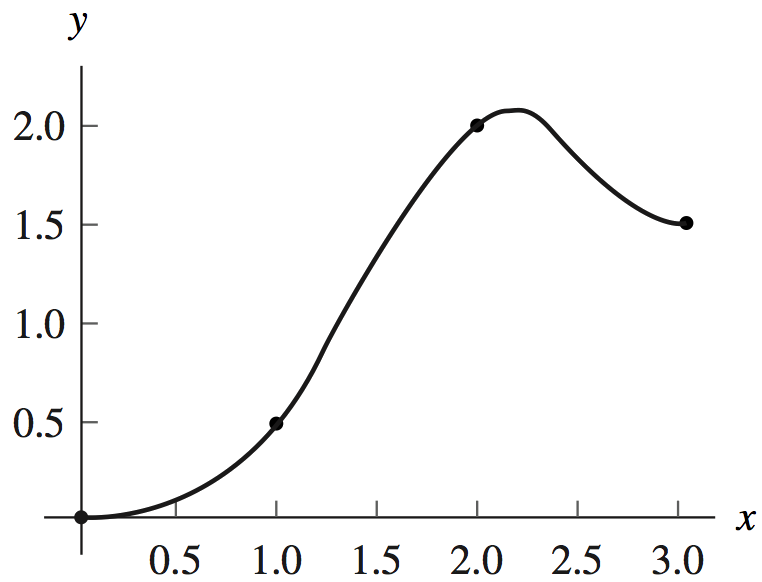
\includegraphics[width=40mm]{chap-4/fig_5-16.png}
\end{center}
\end{figure}
}



\frame{
\frametitle{ Suitability of Cubic Splines }
\framesubtitle{三次样条的适配性}
\begin{itemize}
\item A practical feature of splines is the minimum of the oscillatory behavior that they possess. 
\vspace{0.5cm}
\item Consequently, among all functions $f(x)$ that are twice continuously differentiable on $[a,b]$ and interpolate a given set of data points $\{ x_k,y_k)\}^N_{k=0}$, the cubic spline has less wiggle. 
\end{itemize}
}

\frame{
\begin{block}{Theorem (Minimum Property of Cubic Splines).} 
Assume that $f \in C^2[a,b]$ and $S(x)$ is the unique cubic spline interpolant for $f (x)$ that passes through the points
$\{(x_k , f (x ))\}_{k=0}^N$ and satisfies the clamped end conditions $S'(a) = f'(a)$ and $S'(b) = f'(b)$. 
Then
\begin{equation*}
\int_{a}^b \left( S''(x) \right)^2 dx \le \int_{a}^b \left( f''(x) \right)^2 dx
\end{equation*}
\end{block}

Proof \\
Use integration by parts and the end conditions to obtain
\begin{equation*}
\begin{array}{l}
\int_a^b S''(x) (f''(x) - S''(x)) dx \\
= S''(x) (f'(x) - S'(x)) |_{x = a}^{x = b} - \int_a^b S'''(x) (f'(x) - S'(x)) dx \\
= 0 - 0  - \int_a^b S''(x) (f'''(x) - S'(x)) dx
\end{array}
\end{equation*}
}

\frame{
 Since $S'''(x) = 6_{s_{k,3}}$ on the subinterval $[x_k , x_{k+1}]$, it follows that
\begin{equation*}
\int_{ x_k}^{x_{k+1}} S'''(x)( f'(x) - S'(x)) dx = 6_{s_{k,3}}( f (x) - S(x)) |^{x=x_{k+1}}_{x=x_k} = 0
\end{equation*}
for $k = 0, 1, \ldots,N-1$.
Hence $\int_a^b S''(x) ( f''(x) - S''(x)) dx = 0$, and it follows that
\begin{equation*}
\int_a^b S''(x) f''(x) dx = \int_a^b \left( S''(x) \right)^2 dx
\end{equation*}
}

\frame{
Since $0 \le ( f''(x) - S''(x))^2$, we get the integral relationship
\begin{equation*}
\begin{array}{l l}
0 & \le \int_a^b ( f''(x) - S''(x))2 dx \\
   & = \int_a^b ( f''(x))^2 dx - 2 \int_a^b f''(x)S''(x) dx + \int_a^b (S''(x))^2 dx.
\end{array}
\end{equation*}
Now the result  is substituted into (4.74) and the result is
\begin{equation*}
0 \le \int_a^b (f''(x))^2 dx - \int_a^b \left( S''(x) \right)^2 dx
\end{equation*}
}





\frame{
\begin{itemize}
\item The following program constructs a clamped cubic spline interpolant for the data points $\{ (x_k, y_k) \}f^N_{k = 0}$ 
\item The coefficients, in descending order, of $S_k(x)$, for $k = 0, 1, ... , N-1$, are found in the $(k -1 )$st row of the output matrix $S$. 
\item In the exercises the reader will be asked to modify the program for the other endpoint constraints listed in Table  and described in Lemmas 2 through 5.
\end{itemize}
}



